\documentclass[11pt,a4paper]{article}
\usepackage[lmargin=1in,rmargin=1in,tmargin=1in,bmargin=1in]{geometry}
\usepackage[pagewise]{lineno} %line numbering
\usepackage{setspace}
\usepackage{ulem} %strikethrough - do not \sout{\cite{}}
\usepackage{xcolor} %change font color
\usepackage{graphicx}
\usepackage{filecontents}
\usepackage{tablefootnote}
\usepackage{footnotehyper}
%\usepackage{subfig}
\usepackage[yyyymmdd]{datetime} %date format
\renewcommand{\dateseparator}{.}
\graphicspath{{../img/}} %path to graphics
\setcounter{secnumdepth}{5} %set subsection to nth level
\usepackage{caption}
\captionsetup[table]{skip=11pt} %sets a space after table caption
\usepackage{times}
\usepackage{tabto} %general tabbed spacing
\usepackage{longtable} %need to put label at top under caption then \\ - use spacing
\usepackage[stable,hang,flushmargin]{footmisc} %footnotes in section titles and no indent
\usepackage[round]{natbib} %parenthesis instead of brackets for inline citations
\usepackage{enumitem}
\usepackage{boldline}
\usepackage{makecell}
\usepackage{booktabs}
\usepackage{amssymb}
\usepackage{amsmath}
\usepackage{physics}
\usepackage{tabularx}
\usepackage{multirow}
\usepackage{lscape}
\usepackage{array}
\usepackage{caption}
\usepackage{subcaption}
\usepackage[labelfont=bf]{caption}
\usepackage{chngcntr}
\usepackage{hyperref}

%\counterwithin{table}{section}

%\usepackage{xr}
%\externaldocument{} %aux file needed

\newcommand{\edit}[1]{\textcolor{blue}{#1}} %shortcut for changing font color on revised text
\newcommand{\fn}[1]{\footnote{#1}} %shortcut for footnote tag

\newcommand*\sq{\mathbin{\vcenter{\hbox{\rule{.3ex}{.3ex}}}}} %makes a small square as a separator $\sq$

\usepackage{fancyhdr}
\pagestyle{fancy}
\fancyhf{} %move page number to bottom right
\renewcommand{\headrulewidth}{0.5pt} %turn off line in header
\lhead{\scriptsize Prof. R. A. Borrelli} 
\rhead{\scriptsize \today}
\rfoot{\thepage}

\begin{document}

\begin{titlepage}
    \title{
        \textbf{MCNP for Engineers}\\
        A walkthrough on how to use it, get results,\\
        and\\
        What it all means to a fulfilling life
    }
    \author{
        Prof. R. A. Borrelli
        \\ \\ \\
        University of Idaho $\sq$ Idaho Falls Center for Higher Education\\
        Center for Advanced Energy Studies\\[0.05in]
        Engineering/Technology Management, Industrial Technology\\and\\Nuclear Engineering Department
        \\ \\ \\
        rborrelli@uidaho.edu
        \\ \\ \\
        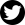
\includegraphics{twitter.png}
\includegraphics{git.png}\\
        @TheDoctorRAB\\ \\
    }
\clearpage %not have page number on title page
\maketitle
\thispagestyle{empty} %start with page number 1 on second page
\end{titlepage}

\chead{\scriptsize \textit{MCNP walkthrough - Preface}}

\section{Preface} \label{preface}
\subsection{Who is this walkthrough for?}
\noindent Advanced undergraduate students and graduate students in any nuclear engineering curriculum. Students should know - 
\begin{itemize}[topsep=0pt,itemsep=-1ex,partopsep=1ex,parsep=1ex]
    \item Basic nuclear physics; e.g., cross sections
    \item Interactions of neutrons and photons with matter
    \item Shielding, dose rates
    \item Four/six factor formula; e.g., what $k_{EFF}$ is,
    \item How a nuclear reactor works
    \item Solving for buckling
    \item Neutron diffusion
\end{itemize}
\vspace*{\baselineskip}

\noindent Just about every nuclear engineering department has this course. Typically, the Lamarsh or Duderstadt textbooks are used mostly. Sometimes the Shultis textbook is used. It's usually one of the first classes taken prior to the higher-level nuclear engineering courses. However, this course provides all you need to know to run and understand MCNP. I happen to teach this course. I use Lamarsh with Shultis as a reference. I happened to use Lamarsh because that was the textbook when I first took this kind of course. There really is no argument for one over the other.

\subsection{What is MCNP?}
\noindent Your best friend. Your greatest nemesis. MCNP is a contradiction. It will make you suffer, but it will open doors and present new opportunities. \\

\noindent MCNP is a computational tool - that means you're not coding \textit{per se}. You set up the input file that the code will read and then execute. MCNP tracks neutrons and photons for specified geometries and produces a wealth of resulting data. That seems simple. It's not. With a little guidance, effective modeling with MCNP is achievable. 

\subsection{Why is MCNP so important?}
\noindent It's not that necessarily MCNP itself is so important. Neutronics modeling is. We can't design any reactor without knowing where the neutrons are going and what they're going to do when they get there. MCNP happens to be the first neutronics computational tool. (They literally used punch cards.) All other tools are benchmarked against MCNP.\\

\noindent Not everyone is going to be a neutronics expert. For those that want to be, mastering MCNP makes it far easier to learn other neutronics codes, like Serpent. Any facility with MCNP provides a fundamental basis for a career in nuclear engineering. Frankly, if you're a graduate student, you're looking for internships. You may not really care what you're going to do; you just want a good position for your CV and a chance to network for future career development. Absolutely nothing wrong with that. On more than one occasion, I have had a researcher come up to me and ask `Do you know any of the students that know MCNP? I have some money for an intern this summer, but I need someone to step in and get right going.' I intend for this walkthrough to give you the skills to step right in and get going.\\

\noindent Learning MCNP will also lend to transferable skills. Whether it is good coding practices, geometric modeling, or just developing engineering judgement, this will lead to success in higher endeavors. \\

\newpage

\chead{\scriptsize \textit{MCNP walkthrough - Motivation}}

\section{Motivation - Do we \textit{really }need another `How to use MCNP'?} \label{motivation}
\subsection{Maybe?}
\noindent Don't read this if you don't want to. I'm not losing sleep over it. Due to the virus sweeping the nation in 2020, over the summer, I decided I needed to take the time to prepare my fall course with the contingency for shifting to online delivery. I've taught the course since 2015, so I know the material, have all the slides and assignments, etc., already prepared. This is part of that effort. Students should be able to follow this on their own and learn how to use MCNP. 

\subsection{An embarrassment of riches}
\noindent There are tons and tons and tons and tons of MCNP resources floating around out there. I have compiled them as I find them in my \href{https://courses.lumenlearning.com/uidaho-nuclear/}{Online educational resources for nuclear engineering.} However, all this decentralization just spreads the materials out so much that there isn't really an orderly way to work through them as a learning process. There are a lot of good problems out there that I use in class. \\

\noindent Probably the closest resource to what I'm trying to do here is the famous \href{https://www.mne.k-state.edu/~jks/MCNPprmr.pdf}{MCNP primer} from Prof. Shultis at Kansas State University. A particularly good feature of the primer is that it cross references to the MCNP manual. I certainly used it when I first learned MCNP. However, I do not know if that manual is shipped with MCNP anymore, and the most recent revision of the primer that I have found is 2011. To be fair, not too much has changed in the ensuing time, but just about all of the resources in addition to the primer that I have found are somewhat dated. The time seems right to develop something new. Another difficulty I have is that most of these resources are gigantic information dumps. It was overwhelming for me when I was first learning MCNP. I like writing, I'm fairly good at it, and given the context of 2020, the time felt right to give this a shot. \\

\newpage

\chead{\scriptsize \textit{MCNP walkthrough - Personal}}

\section{Experience - And who do you think you are?} \label{experience}
\noindent Well, I'm an actual nuclear engineering professor. I've taught the Lamarsh class with an MCNP learning module every year since 2015. Students have attained solid success with publications, internships, and gainful employment from the course. I have many publications applying MCNP in a variety of topics. My expertise in MCNP has led to several funded projects. Ask about me. \\

\noindent I am by no means the leading expert in MCNP. I'm probably not a leading anything unless I'm leading you to happy hour. I can name probably 12 - 15 people I know personally that are better at neutronics modeling than me. However, actually \textit{teaching} MCNP formally is a different paradigm, altogether. I am confident that I'm on a short list of being able to teach \textit{how to use MCNP effectively}. I am purposely very specific in claiming what I can actually do here. 

\section{Style - What's wrong with you?}
\noindent Plenty, but now's not that time for that. \\

\noindent As you may have gathered so far, my tone is intended to be conversational and not overly ponderous. So, not like a journal paper. I'm writing in the way I have been lecturing on MCNP. I'm trying to ease you through the learning process and not just dump everything on to the page. I'm not trying to talk down to anyone. I know the difficulties I had with learning MCNP, so I'm writing in a way that I would have wanted to be spoken to. Even that's a bad sentence, but this isn't meant to be a formally reviewed and published document.\\

\newpage

\chead{\scriptsize \textit{MCNP walkthrough - Intent and direction}}

\section{Teaching MCNP for \textit{engineers}}
\noindent There is a reason why I chose the title that I did. I'm interested in getting students and other researchers the guidance they need to run MCNP. If I were going to prepare a course, then, sure, I would spend a significant time on Monte Carlo theory. And I'll have a brief section in here about that. I'm not arguing that a scientific approach isn't valuable in comparison to engineering. I have found most MCNP resources include a ton of material on the theory behind MCNP. I'm assuming you know that already. If you feel like you need some background on the theory behind MCNP, I direct you to \href{https://laws.lanl.gov/vhosts/mcnp.lanl.gov/pdf_files/la-ur-05-4983.pdf}{Fundamentals of Monte Carlo particle transport} by Dr. Forrest B. Brown at Los Alamos National Laboratory. If there's only one expert in MCNP and Monte Carlo theory, he is probably that person. 

\section{\textit{Walkthrough}}
\noindent I also chose the term `walkthrough' deliberately. Here's where I think I bring some value versus other resources. When I think about a walkthrough, I'm thinking about video games - You're playing a cool game but for the last hour you're stuck in a room looking for a lever or loose tile or you're asking questions to the townspeople and you know you have to do it in a certain order but you're going in circles. The game is starting to get tedious and you need a hint. The walkthrough provides a detailed account of the game - right down to where to look or, not only what weapon to select, but what move to employ. That's what I'm going for here - `Fatal error? Look up.' MCNP is slightly more complex than a video game, but if you can build an input file from scratch and get it to run, then you're well on your way. Building in more complexity isn't as overwhelming. 

\newpage

\chead{\scriptsize \textit{MCNP walkthrough - Getting started}}

\section{Installation}
\noindent Detailed installation instructions are provided with your MCNP disks. I am not going to repeat them here, but you should follow them to the letter. Run the tests after to make sure everything is all set. Remember, your license only allows you to install MCNP in one place due to export control restrictions. Mine is on my office desktop. I do not recommend installing it on a laptop. If it gets stolen, you could get into some trouble. Your license is granted through your institution. If you change positions and go somewhere else, then you need to apply for another license and you have to uninstall the distribution under the prior license and destroy the disks. 

\section{Operating system}
\noindent I strongly recommend installing in linux. Over the years, I've experienced either first hand or with students, inexplicable wonkiness with MCNP in a Windows environment. Don't have a linux system? No problem! You can install a `virtual linux machine' on your windows computer. It takes some time, but it's not hard. I have MCNP installed on the virtual machine in my office. I am using the `Oracle VM VirtualBox Manager'. That is basically the holder for your linux environment. I use the CentOS8 linux system. There's others to choose from. If you have the computing power, you can have the box make two screens or more if you have a multiple monitors. I actually use the linux box about 99\% of the time for MCNP, data processing, lecture slides, presentations, papers, all of it. 

\section{Visualization}
\noindent The linux distribution for MCNP comes with a plotter equipped to view your models. There's nothing extra to do in a standard linux environment. MCNP used to ship VisEd. I started on VisEd, so I am more used to it than the plotter. Both aren't super great. VisEd only runs in windows. You can request a VisEd download separately after you obtain your MCNP license. I would recommend it. Try both. It's kind of a pain to copy your MCNP file from linux to windows, but it's not really that bad.

\section{Text editor}
\noindent MCNP is a FORTRAN code. \textit{FORTRAN}. That's an old language. O. L. D. That means you have to be really careful in your selection of a text editor. FORTRAN will go sideways fast if there's any whitespace or `$\wedge M$' in there. It is also very column specific. This is because when they first invented the language, they were programming on punch cards. Fortunately, there are plenty of choices in linux that can be used to build your input files. I use \texttt{vim}. I started on \texttt{vi}
at an internship in undergrad at the Naval Undersea Warfare Center because the particular group I was working in used that. I actually learned FORTRAN there. The other popular editor is \texttt{emacs}. In linux, there are many choices. Use one of these. 

\section{Scientific computing best practices}
\subsection{Python}
\noindent As a nuclear engineering graduate student, I know you all have a copy of \href{https://www.google.com/books/edition/Effective_Computation_in_Physics/6IkNCgAAQBAJ?hl=en&gbpv=0}{Effective Computation in Physics: Field Guide to Research with Python}. This book, and I feel like using the term `book' to describe this treatise to a successful research career just falls short, should be your guide to best computing practices. Again, installing MCNP in linux allows for more ready
postprocessing with the accessibility to python. You can install python in your windows environment, but I just find installing packages to be a lot easier in linux. 

\subsection{Postprocessing}
\noindent For more complex neutronics and/or photon modeling, effective postprocessing is a necessity. Fortunately, with python, you can find many scripts to edit for your own purposes. I have several on my github. Please feel free to look around my repositories. Additionally, I've found it easier to prepare graphs in python. I have several python graph scripts as well. MCNP comes with plotting capabilities. I never got around to learning how to use them yet. That doesn't mean they aren't useful.

\subsection{Reproducibility}
\noindent Good computing means your creation can be used by other people. If you make an MCNP file, someone else should be able to run it and produce the same results that you obtained. This provides confidence that you produced research that is scientifically sound. Then, whomever has your MCNP file can modify, enhance, or build upon the model to tackle more problems. We must have this principle in mind when developing MCNP files. As I walkthrough MCNP, I'll make note of this. 

\newpage

scope
\end{document}
